\documentclass{article}
\usepackage[
backend=biber,
style=alphabetic,
sorting=ynt
]{biblatex}
\addbibresource{bibliography.bib}

 \usepackage{graphicx}
\graphicspath{ {./images/} }


\title{Entity Linking Literature Review }
\author{Will Thompson}
\date{October 6, 2022}

\begin{document}

\maketitle

\section{Introduction}

The task of {entity linking} (\url{https://en.wikipedia.org/wiki/Entity_linking}) is to link entity mentions in text to specific identifiers from a knowledge base. To perform entity linking, two sub-tasks are normally required: (1) predicting named entity mentions in text, (2) linking those entity mentions to entities in a knowledge base. It appears to be common to assume that (1) is given, and evaluate a system on (2) alone. Overall performance, however, is clearly dependent on doing well in both steps.

My core interest is in applying entity linking to \emph{clinical notes}, unstructured text that can be found in large quantities in electronic health records (EHR). There is a lot of potentially useful information in such notes, ranging from disease mentions, descriptions of symptoms, past medical history, and on and on. While EHR also have large quantities of structured information, it turns out that such information is often incomplete or even mis-leading. Structured data in the EHR are mostly collected either in direct support of patient care, or for billing purposes -- they are not typically collected to perform secondary analyses such as investigating disease progression, responses to treatment, etc. For example, billing for a medical visit requires the medical facility to submit an ICD-10 code (for diagnosis), and a CPT code (for procedure). But such codes will be issued even for things like \emph{testing} for a particular condition, and if the test is negative, we certainly can't take the ICD-10 code as a true statement about the condition of a patient. Clinical notes often contain a more direct assessment of a patient's condition, and is typically the only place where information like medical symptoms and past medical history is stored.

There are two highly salient background facts relevant to clinical NLP. First, there is general lack of labelled data. Due to privacy concerns and regulations (prominently, HIPAA), there is not much in the way of shared corpora, much less annotated shared corpora. Second, there is an abundance of knowledge bases, some of which have existed for decades. For example, the Unified Medical Language System (UMLS; \cite{bodenreider_unified_2004}), created by the National Library of Medicine, contains millions of clinically relevant entities, linked into a semantic network. My goal for this literature review is to identify resources that can help with entity linking in the clinical domain, given these two background facts. I would like to be able to do high quality entity linking without much in the way of annotated gold standards, leveraging what little is available to link mentions in clinical notes to resources such as the UMLS.


\section{Reviewed Publications}

% --------------------------------------------------------------------------------------------------------------------------------------------------------------------------------------------
\subsection{\cite{schumacher_clinical_2020}: \citetitle{schumacher_clinical_2020}}

\begin{figure}
\centering
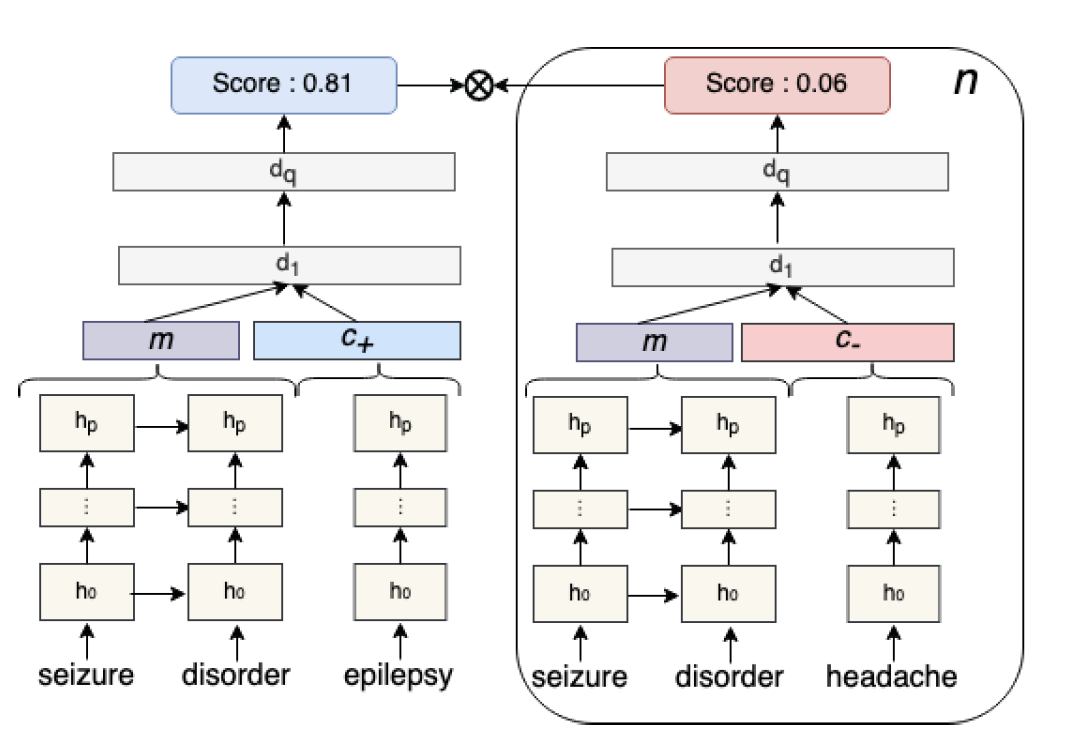
\includegraphics[scale=0.5]{clinical-concept-linking-fig-1}
\caption{from \cite{schumacher_clinical_2020}}
\label{fig:concept-linker}
\end{figure}

\subsubsection{Problem}

This paper motivates the task of \emph{concept linking}, which they describe as adjacent to (but not quite the same thing as) \emph{entity linking}. The primary distinction is that concept linking lacks the descriptive content that entity linking typically takes advantage of. Concepts come with identifiers, links to synonyms and related concepts, but rarely long-form text. This is relevant in the clinical space because this is what characterizes the ontologies/terminologies that are typically available here. Therefore, concept linking relies on (1) local context from the mention, and (2) whatever information is available in the ontology. This is unlike something like Wikipedia, where each page can be taken as an extensive long-form description of a particular entity. The authors also describe the lack of annotated data in the clinical space, due to the issues outlined in the introduction of this literature review. Their approach is informed by these resource limitations.

\subsubsection{Approach}

The concept linker described in the paper consists of a pairwise neural network ranker using contextualized  representations for both the mentions and the concepts. For a given entity mention and document, the ranker ranks all possible candidate concepts in the knowledge base. Training is done with pairwise loss, with two networks, one which takes the mention and the correct concept, and another which takes the mention and an incorrect concept  (see Figure \ref{fig:concept-linker}). The contextualized representations use an RNN approach (ELMo), trained on clinical notes from the MIMIC 3 note corpus. Mention representations are extracted as the lowest token representation from the LSTM. Concept representations are trained on the concept names. The model is pre-trained on all concept names, synonyms, and definitions from the UMLS for the relevant subset of the UMLS for which they have annotated data. The annotated data is from a shared evaluation task (ShARe/CLEF eHealth Evaluation Lab 2013 Task), which made use of MIMIC 2.5 clinical notes, annotated with UMLS disorder concepts.


% --------------------------------------------------------------------------------------------------------------------------------------------------------------------------------------------
\subsection{\cite{dong_ontology-based_2022}: \citetitle{dong_ontology-based_2022}}

\subsubsection{Problem}

The authors address the issue of extracting rare disease entities from clinical text. Rare diseases are those affecting $\leq 5$ people in $10,000$. While each such disease is (by definition) rare, there are many such diseases, therefore having a rare disease is not exactly rare. There are very few annotated resources for such conditions (a common refrain for clinical NLP in general), which is the essential challenge the authors are trying to overcome. They also discuss mapping between two ontologies (from UMLS to ORDO), but this latter concern is out of focus for this literature review, and I'll focus on the entity linking portion of the paper.

\subsubsection{Approach}

The core ideas are to use weak supervision combined with contextualized mention representations (BERT). They use a rules based method to generate relatively high quality mention/entity pairs, which can be used to then train a classifier over contextualized representations. The rules consist of string matching to concepts in the UMLS ontology, followed by a filtering step to remove many false positives. One filtering rule, for example, is to exclude mentions that are ``too short'', as such mentions are frequently highly ambiguous. The training data was derived from discharge summaries in the MIMIC 3 corpus. A smaller set of notes was hand annotated to produce a gold standard for evaluation purposes. For the contextual language model, they used a pre-trained BERT model trained on clinical notes.


% --------------------------------------------------------------------------------------------------------------------------------------------------------------------------------------------
\subsection{\cite{logeswaran_zero-shot_2019}: \citetitle{logeswaran_zero-shot_2019}}

\subsubsection{Problem}

Zero-shot entity linking: linking mentions to unseen entities without in-domain labeled data. An example they give, is linking to specialized dictionaries such as legal cases, company project descriptions, characters in a novel. Labeled data probably not readily available, and it is expensive to create such resources. The goal of the paper is to build an entity linking system that can generalize to new domains without labeled training data.

\subsubsection{Approach}

They outline three contributions in the paper:

\begin{enumerate}
\item Proposing a new zero-shot entity linking task, and constructing a public dataset for this task using documents from Wikia.
\item Building a strong baseline with a BERT-based reading comprehension model, with attention layers on concatenated mentions in context + entity descriptions
\item An adaptation strategy they call \emph{domain adaptive pre-training} (DAP) that further improves entity linking performance.
\end{enumerate}

They drop the normal assumptions of entity linking approaches, and assume only the weaker assumption that we have an \emph{entity dictionary} $\mathcal{E} = \{(e_i,d_i)\}_{i = 1,...,K}$ where each $d_i$ is a text description of entity $e_i$. They assume the presence of labeled data for training, including documents with labeled mentions, and gold standard entities attached. There is no such assumption for the target data, just an entity dictionary as described above. They adopt a 2-stage pipeline for entity linking. First is a fast candidate generation stage, followed by a more expensive BERT-based candidate ranking stage. Candidate generation uses an information retrieval approach, using BM25 to pull out the top-k (k = 64 in their experiments) to pull out candidate mentions from texts. Candidate ranking is done with a transformer model which concatenates the candidate mention text with the entity descriptions. They refer to this as the \emph{Full Transformer} model. Their final step is to use DAP, as mentioned above. They pre-train the model on text first on open corpora (Wikipedia and BookCorpus for this experiment), followed by source and target text, followed by just target text, before training on the labeled source data. Compared to baselines, the best performance on unlabeled target data was achieved using Full Transformer + DAP. Evaluation metric was average top-1 accuracy.


% --------------------------------------------------------------------------------------------------------------------------------------------------------------------------------------------
\subsection{\cite{wu_scalable_2020}: \citetitle{wu_scalable_2020}}


\begin{figure}
\centering
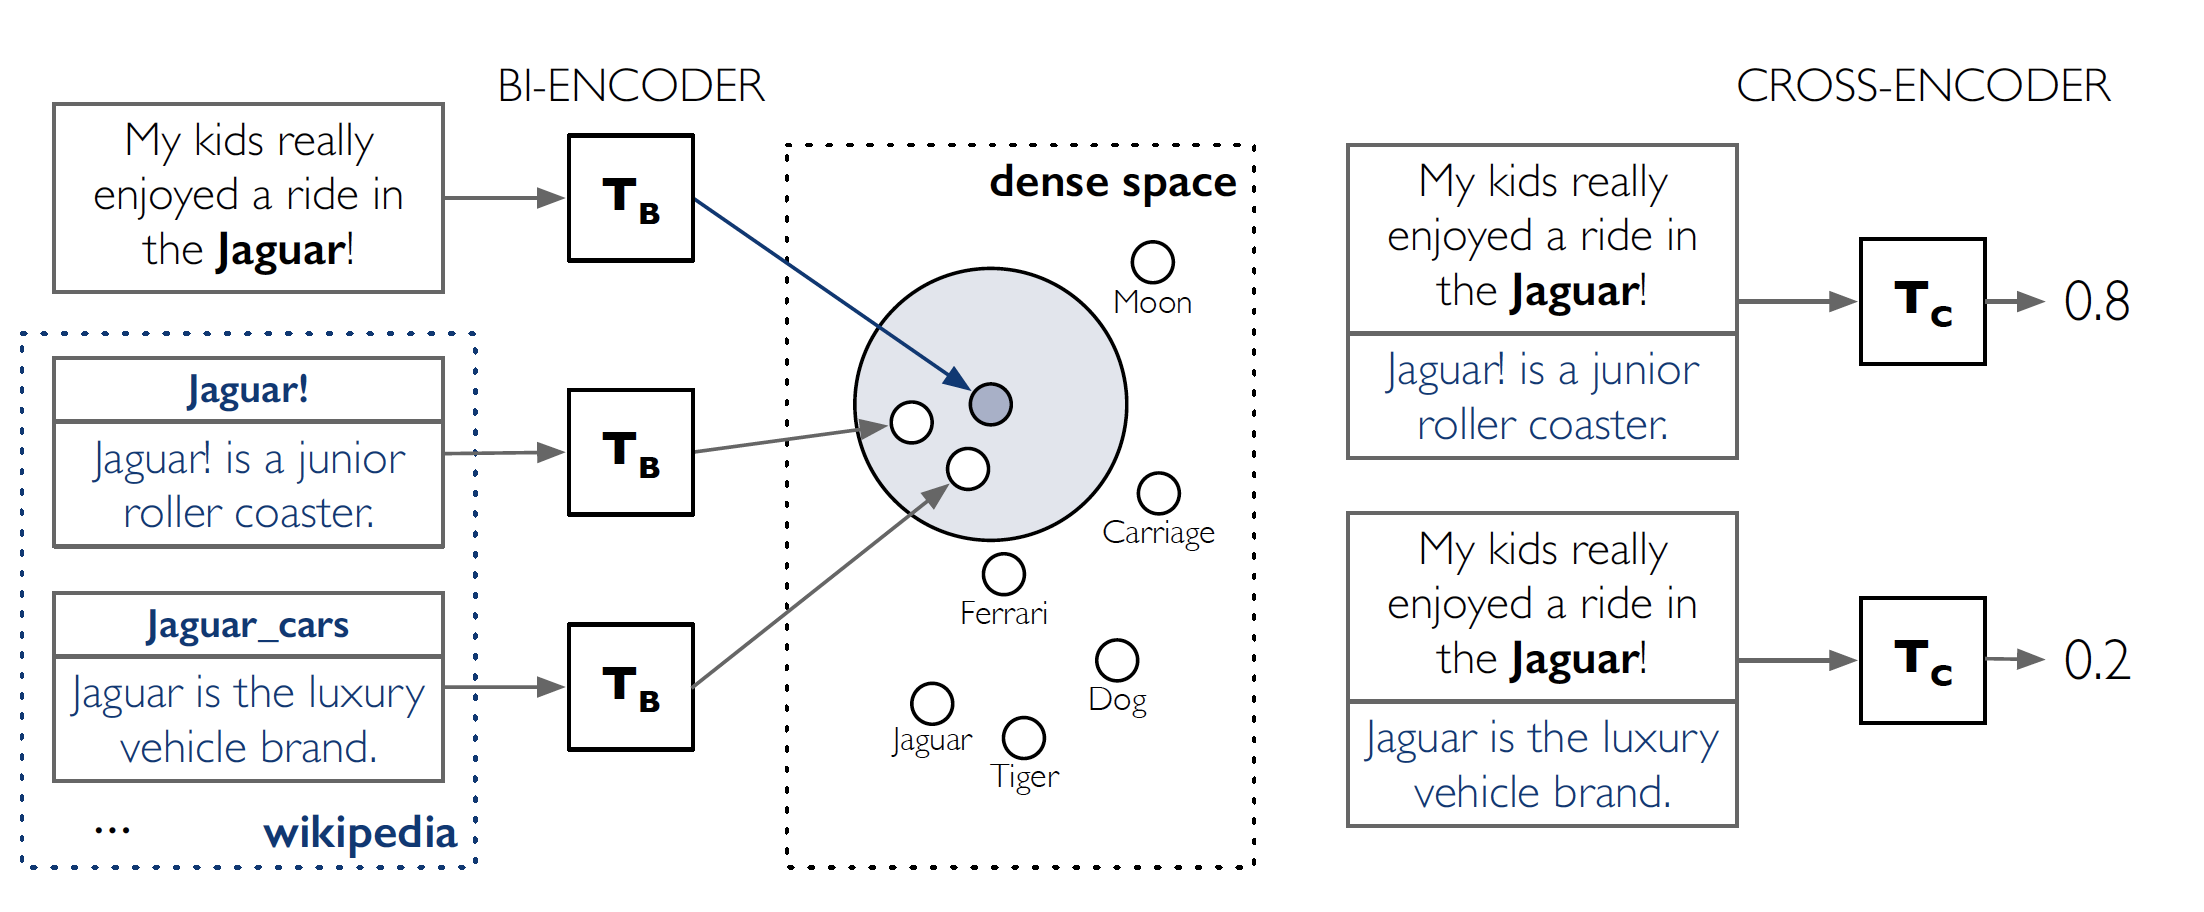
\includegraphics[scale=0.33]{zero-shot-fig-1}
\caption{from \cite{wu_scalable_2020}}
\label{fig:zero-shot}
\end{figure}

\subsubsection{Problem}

This paper develops zero-shot entity linking further, following \cite{logeswaran_zero-shot_2019}.  The zero-shot problem statement is the same as above, but they add the additional goals of scalable candidate generation using a BERT-based dense encoding model.

\subsubsection{Approach}

The standard assumption is made that entity mentions come pre-annotated. They then follow \cite{logeswaran_zero-shot_2019} in adopting a two stage approach (see Figure \ref{fig:zero-shot}). The entity mentions and entities each get encoded into the same dense vector space using . Dot-product similarity is then used to find the top-k candidate entities for a given entity mention. A crossencoder is used to rank the candidates. Again similar to \cite{logeswaran_zero-shot_2019}, the crossencoder is given concatenated representations -- the entity mention is concatenated with the candidate entity representation.

% --------------------------------------------------------------------------------------------------------------------------------------------------------------------------------------------
\subsection{\cite{du_entity_2022}: \citetitle{du_entity_2022}}

\begin{figure}
\centering
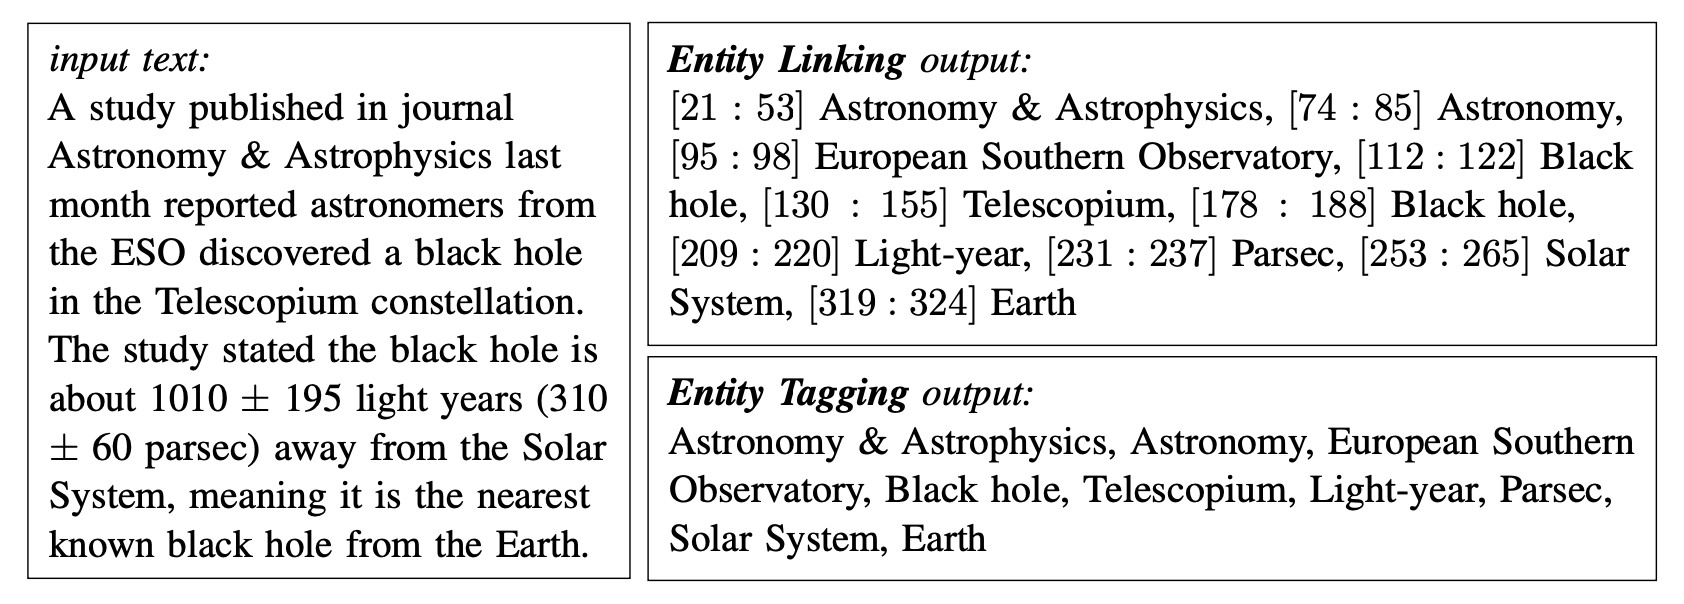
\includegraphics[scale=0.5]{entity-tagging-fig-1}
\caption{from \cite{du_entity_2022}}
\label{fig:entity-tagging}
\end{figure}

\subsubsection{Problem}

What if we could do entity linking without entity mention detection? Do we really need to bother with that first step? There are lots of applications where we just need the entities identified, no need to demarcate the precise strings of text where they are evoked. Instead of a 2 stage pipeline, the authors attempt to create a direct mapping from text to entities (see Figure \ref{fig:entity-tagging}).

\subsubsection{Approach}

Framing \emph{entity tagging} as a sequence-to-sequence problem, the propose an autoregressive model that generates a set of entity names given an input sequence (GET: \emph{Generative Entity Tagging}). Training setup consists of a input text and a corresponding set of gold entities, concatenated in random order. The model is trained to optimize the probability of the output sequence (the concatenated set of entities). (Note: I don't really understand what the point of the random permutation is. If I end up making use of ideas from this paper, this is an area I'll have to delve into more deeply). At prediction time, the model chooses the most likely next token at each decoding step. At the end, this sequence of tokens is split by the separator token, and then converted into a set of entities. Training data consists of news articles (AIDA dataset), annotated with entities from a knowledge base, as well as Wikipedia articles with partially annotated mentions. Evaluation is performed on AIDA, as well as other corpora. Evaluation metrics are precision, recall, and F1 score vetween the set of ground truth entities and the predicted entities. The GET model is based on pre-trained T5-base architecture and trained with cross entropy loss to maximize the likelihood of the target sequence. The results obtained were as good as (and mostly a bit better than) an existing AIDA-trained entity linking model, demonstrating that labeled entity mentions are not required in order to achieve good performance in predicting entities directly from unlabeled text.

% --------------------------------------------------------------------------------------------------------------------------------------------------------------------------------------------
\section{Discussion}

\cite{schumacher_clinical_2020} formulates the entity linking task in the context of clinical notes, and the typical resources available in this context. This includes a general lack of high-quality annotated data, but the general availability of large medical ontologies. In this regime, they call the task \emph{concept linking}.  This paper motivates the use of contextual language models for this task, and outlines some of the challenges to applying those other systems to entity linking for clinical notes. It is a useful baseline to compare with some of the other systems described below.

\cite{dong_ontology-based_2022} motivate the use of weak supervision to create classifier training data. This idea could prove quite useful in the context of the two papers that address \emph{zero shot} entity linking. In particular, \cite{logeswaran_zero-shot_2019} explicitly mentions that adding a weak supervision step would be a potential way to improve on their results. My main take aways from \cite{dong_ontology-based_2022} are some ideas for doing weak supervision in the context of these zero shot approaches. This may turn out to be one of the core innovative steps for my final project.

\cite{logeswaran_zero-shot_2019} presented a very interesting idea, treating candidate generation as an information retrieval task. I'm hopeful that I can make use of this core idea for my project. One issue, however, is that medical resources such as UMLS do not have much accompanying text (as described in \cite{schumacher_clinical_2020}). It's not like wikipedia, where each article can be taken as a description of an entity. So this is something that would have to be figured out in order to adapt this idea to the clinical space. Perhaps it would be possible to use the semantic network of UMLS to create an artificial context of clusters of concepts which are likely to co-occur as mentions in a document. This could be an avenue of exploration and experimentation.


Compared to \cite{logeswaran_zero-shot_2019}, the candidate generation approach in \cite{wu_scalable_2020} resulted in a significant improvement. The first-stage candidate generation using the transformers had much better recall than the BM25 algorithm used in  \cite{logeswaran_zero-shot_2019}, and \cite{wu_scalable_2020} gets much higher accuracy using the same Wikia dataset. \cite{wu_scalable_2020}  therefore appears to be a clear improvement over \cite{logeswaran_zero-shot_2019}. It would be a great experiment to see how much of this can be applied to the clinical entity linking problem.

The entity tagging idea described in \cite{du_entity_2022} is very intriguing, as it removes any need for mention annotations. I think this would be applicable to many applications of clinical entity linking. Sometimes we just need the entities. For example, we might need to ask if a pathology note asserts the presence of invasive breast cancer. Or if a chest radiograph note indicates that a patient has pneumonia. It doesn't necessarily matter where in the text that condition is indicated. I remain uncertain how this idea could be married to the zero shot frameworks described above, but will give it some hard thought.

% --------------------------------------------------------------------------------------------------------------------------------------------------------------------------------------------
\section{Future Work}

Combining my thoughts from the previous sections, there are several tasks that need to be done.

\begin{enumerate}
\item First, I need a corpus of clinical notes. I currently have access to the MIMIC 3 note dataset, which required proper human subjects training. Physionet (the organization that distributes this dataset) also makes available some other corpora, including a collection of radiology notes. I will be looking closely at these to see which might be the most useful for this project. I will certainly need some annotated data for training and testing! Another option is to use biomedical literature data -- the \emph{MedMentions} corpus consists of a collection of biomedical paper abstracts annotated with UMLS concepts. While not clinical notes, this might be one way to try out approaches on a related set of data.
\item Obtain and set up the UMLS ontology. It is quite large, with millions of concepts. I have the required account with the National Library of Medicine already, but this will need some work to figure out how to extract the information I will need, such as concept names, descriptions, and links to synonyms and other concepts.
\item Set up a baseline system. My current thought is to start with \cite{wu_scalable_2020}. They have open sources their code on github (\url{https://github.com/facebookresearch/BLINK}). Getting this working will take some effort. Then translating it to the clinical/UMLS world will take some effort.
\item Implement an innovative step. I'm thinking of trying out ColBERT for information retrieval of candidate entities, as well as using weak supervision to improve performance in a target domain.
\end{enumerate}

This is all quite daunting, but I'm excited to see if I can make it work!

% --------------------------------------------------------------------------------------------------------------------------------------------------------------------------------------------
\medskip
\printbibliography
\end{document}
